\documentclass[11pt]{article}

\usepackage[english]{babel}

\usepackage{langsci-gb4e}
\usepackage{graphicx}

\usepackage{unicode-math}
\usepackage{fontspec}
\usepackage{libertine}
\setmathfont[Scale=MatchUppercase]{Libertinus Math}
\setmonofont{Inconsolata-g}

\usepackage[backend=biber,
	natbib=true,
	style=biblatex-sp-unified,
	citestyle=sp-authoryear-comp,
	maxbibnames=99,
	isbn=false,
	doi=false,
	eprint=false
]{biblatex}
%\addbibresource{BigBiblio.bib}

% corex_biber.bib was created automatically by running
% `biber --output_format=bibtex --output_resolve corex.bcf`
% DO NOT MODIFY MANUALLY

\addbibresource{corex_biber.bib}

\title{Automatic register annotation?}

\begin{document}
\maketitle
\section{Alternation modelling and register classification}

\subsection{Corpus-based modelling of linguistic variation}

Modelling linguistic variation in the broadest sense is clearly one of the major goals -- if not \textit{the} major goal -- of linguistics.
Speakers trivially do not use the same expressions for non-identical content (compositional semantics) or communicative intent (pragmatics).
They do not use the same expressions even for the same content or communicative intent in different regions (regio- or dialect), different social groups (sociolect), or based on individual preference (style).
Furthermore, speakers use different forms in different communicative settings (such as talking to close personal friends vs.\ giving a talk in the process of applying for a tenured academic position), which is what we understand as \textit{register}.
Linguistic variation -- even under a fairly traditional view -- thus occurs at the level of individual utterances (driven by semantics and pragmatics), the level of individual speakers (style), the level of groups of speakers (dialect and sociolect), and the within-speaker level (style).
Furthermore, usage-based approaches, which have been on a powerful rise for fifteen to twenty years now, stress that the distribution of concrete forms in utterances is also driven partially by input co-occurrence frequencies.
Under this view, variation is also biased by the fact that some forms happen to be more frequently used together than others, be it for obvious functional or less transparent or obscured reasons.
Speakers most likely also chose their forms partially based on such co-occurrence preferences.%
\footnote{It is clear at this point that all dimensions of variation might overlap and be difficult to disentangle.
Also, variation based on co-occurrence frequencies does not represent an independent dimension of variation as long as there is a transparent functional motivation for a co-occurrence preference.
However, the usage-based perspective adds a stochastic and input-based tone to the picture.}
Finally, random variation should also be expected, either as an effect of so-called \textit{performance} (\ie, production errors based on processing limitations) or because the linguistic system itself (at least as represented in the brains of speakers) does not represent a discrete (traditional linguistic competence) but rather a stochastic system (probabilistic grammar).%
\footnote{Luckily, the heated debate between those two views of random variation in linguistic output is not relevant to this study.}
Modelling linguistic variation thus subsumes the task of specifying why speaker uses the specific expressions that they use under any given circumstances.
Thus, if all sources of variation had been pinpointed and modelled, a full model of human language  would emerge under this broad view.


\subsection{Potentials of incorporating register}



\subsection{The problems with registers in corpora}


\subsection{Statistical issues}



\subsection{Goals and overview}

\cite[vgl.][33--36]{Mueller2010}


% Motivation: Variation, Biber, Bigbert \& automatic register classification based on document-level counts of linguistic features; efforts to automatically generate document-level genre/register meta data based on such data.
% Aim: demonstrate more appropriate use of linguistic features in variational linguistic research;
% Outline: Present Biber-like feature extraction software for German; extract document-level features from corpora of newspaper and web texts; aggregate features via factor analysis; 
% In 3 short case studies of (possibly register sensitive) morpho-syntactic variation phenomena, compare the ``explanatory'' power of the resulting factors to that of (selected) raw features, i.e., not using aggregation. 

\newpage

\section{The COReX feature extractor}

\begin{figure}
  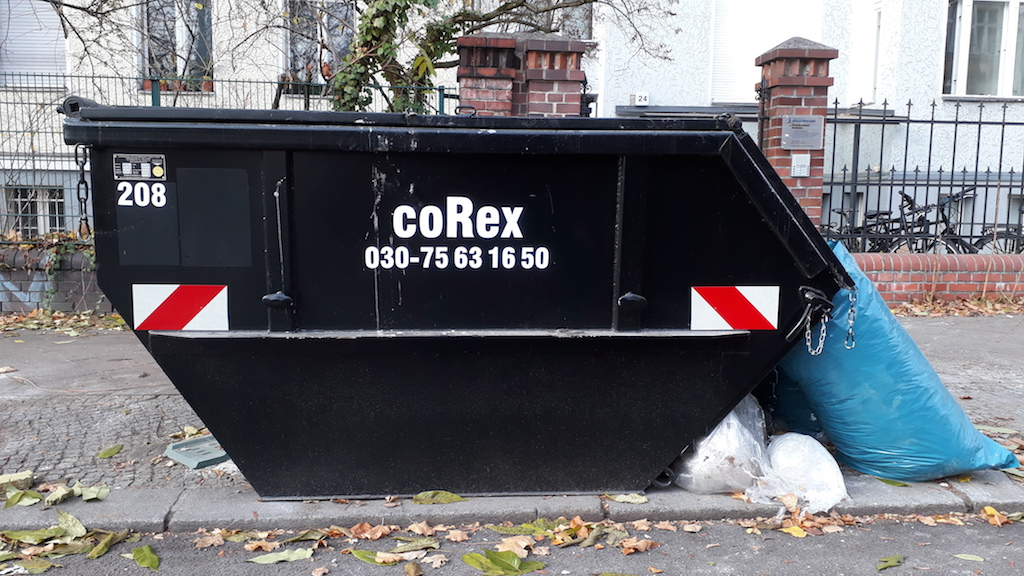
\includegraphics[scale=.3]{corexcontainer.jpg}
  \caption{The COReX feature extractor}  
\end{figure}



COReX is a piece of software designed to extract a large number of normalised feature counts\footnote{Currently, COReX extracts over 60 features. The complete list is provided in the appendix.} at the document level from German text. Most features correspond to linguistic concepts (such as occurrences of a particular parts-of-speech, periphrastic passive and perfect constructions, non-standard morphological forms), alongside a few features which are not strictly linguistic (such as type/token ratio and word/sentence lengths). 
COReX does not perform linguistic annotation by itself, but rather relies on linguistic pre-processing, typically performed automatically by dedicated annotation tools.
COReX is implemented in Python and is easily extendable to include additional features (which, in most cases, will require additional pre-processing of the input corpus).\footnote{Another note.}
%The input format is vertical text (one token per line) with token level annotations in columns 2 through n, and token spans represented as XML-elements (this corresponds to the input format required by tools such as OpenCWB and NoSketchEngine).
%Required XML-elements are doc (document) and s (sentence).

In order to extract the full range of features, the data must include part-of-speech tags (STTS; \citealp{Schiller-ea1999}), morphological features (such as those produced by MarMoT; \citealp{MuellerSchmidSchuetze2013}), named entity annotations (such as those produced by the Stanford NER tagger; \citealp{FinkelGrenagerManning2005}) as well as topological field annotations (as produced by the Berkeley parser; \cite{PetrovKlein2007}, \cite{CheungPenn2009}, \cite{Telljohann-ea2012}).

%For some annotation layers, such as morphological features and topological fields, a particular formatting is required.
%COReX outputs a modified version of the input data where normalised document-level feature counts are added as attribute-value pairs to the opening <doc > tag for each document.
%Moreover, a number of non-normalised counts (such as perfect and passive) are added as attribute-value pairs to the <s > tag for each sentence. Features include non-linguistic categories such as mean word length and mean sentence length; counts for individual parts-of-speech; ...
 
%COReX outputs a modified version of the input data where normalised document-level feature counts are added as attribute-value pairs to the opening <doc > tag for each document.
%Moreover, a number of non-normalised counts (such as perfect and passive) are added as attribute-value pairs to the <s > tag for each sentence. Features include non-linguistic categories such as mean word length and mean sentence length; counts for individual parts-of-speech; ...




[Maybe one or two plots illustrating the distribution of some selected features (e.g., crx\_gen and crx\_prep; or some plots from k-medoid clustering, but this is maybe too much]

\input{clustering}
\section{Feature aggregation}

Information derived from counts of linguistic features in texts can be used in various ways for characterizing the the texts they were extracted from. In pioneering work by \cite{Biber1988},
 \cite{Biber1995}, factor analysis was used to identify a number of ``dimensions of variation'' that could be interpreted in terms of communicative function (such as ``narrative vs.\ non-narrative'', ``involved vs.\ informational production''), and individual texts can then be located at different points on each one of these scales. Contrasting with this multidimensional approach, there have also been attempts to automatically assign texts to single a category (``genre'', ``text type'') based on the occurrence of linguistic features on those texts. An early example of such an approach is \cite{KarlgrenCutting1994}. A recent state-of-the-art example is reported in \cite{EgbertBiberDavis2015}, which illustrates the enormous challenge of automatic register classification on the basis of linguistic feature counts. Using 44 linguistic features in a discriminant analysis for predicting the register category of documents from an ``unrestricted corpus of web documents'', they report precision = 0.342 and recall = 0.396 for their 20 specific sub-registers used in the task (results are generally lower when a smaller number of broader, less specific register categories is used).

In order to explore the effects of feature aggregation in predicting potentially register-sensitive morpho-syntactic alternation phenomena, we use a multidimensional approach (based on Factor Analysis) as described in \cite{Biber1988,Biber1995}. 
In Section~\ref{sec:case-studies}, we will treat the documents' factor scores on each one of the resulting factors as document meta data, and use that meta data in modeling the outcome in specific instances of the alternation phenomenon.
Note that in using a multidimensional approach, we still produce several document-level predictors.
In contrast, assigning each document to a single register category would produce only a single document-level predictor, leading to a greater loss of information.  


\subsection{Factor analysis}

In general, we sought to reproduce the technical aspects of Biber's (1988) study as closely as possible.
There is a major difference, however, in corpus size.
While Biber used material from a total of 481 documents, %(comprising 960,000 words)
 we sampled 70,000 documents from DeReKo and DECOW16B each, totaling 140,000 documents.
Another difference concerns document length.
\cite{Biber1988} imposes an upper limit of approximately 2,500 words per document, whereas we base our counts on whole documents, without an upper limit to the number of words.
The minimum text length is 400 words in Biber's study.
In contrast, we use a lower threshold of only 100 tokens (many documents DeReKo are actually shorter than that).

For the factor analysis, we used a total of 60 feature counts extracted with COReX.\footnote{Absolute counts, such as number of tokens and number of sentences, were discarded.}
The \textit{genitive} count, originally extracted by COReX, was discarded in view of the case study reported in Section~\ref{sec:case-studies}, where the occurrence of genitive is predicted.
 All normalized counts were scaled to z-scores.
 Visual inspection of a parallel analysis scree plot suggested an optimal number of 7 to 8 factors for our data set.
 The plot in Figure~\ref{fa-pa-7-factors} shows the factor loadings from a factor analysis using 7 factors.
 The factoring and rotation methods (\textit{principal factor} and \textit{promax}, respectively) were chosen to match those used and recommended in \cite{Biber1988}.
 
 
\begin{figure}
   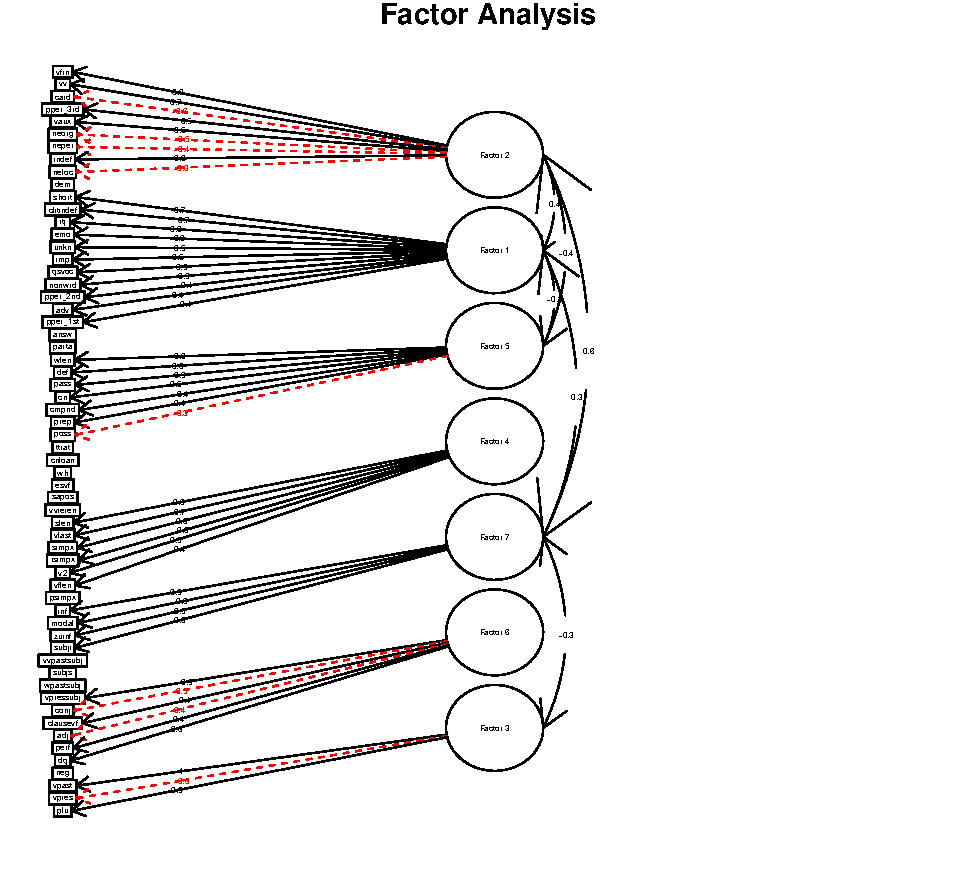
\includegraphics[scale=.9]{../R/fa-fa-7-promax-padded}
   \label{fa-pa-7-factors}
  \caption{Factor loadings of 60 COReX features, from a factor analysis of 140.000 randomly selected documents (DeReKo and DECOW16 combined, minimal document length = 100 tokens), 7 factors, principal factor method, promax rotation. Only the highest factor loading is shown for each feature (loadings < 0.35 are omitted).}  
\end{figure}



Some, but not all of the factors lend themselves to an interpretation in terms of meaningful dimensions of variation.
Most notable among these is Factor~1.
Features with high factor loadings on Factor~1 include short/ contracted forms, interjections, emoticons, imperatives, vocabulary typical of informal written language, as well as first and second person pronouns.
Factor~1 thus most probably captures variability along the lines of formal vs.\ informal, standard vs.\ non-standard, high vs.\ low degree of interaction.
On closer inspection of a number of documents with high scores on Factor~1, it turned out that ``non-standard'' also extends to dialectal texts.
In contrast, finding a plausible interpretation for factors such as Factor~2 is not as straightforward.
Features positively associated with Factor~2 include finite verbs, lexical verbs, auxiliary verbs and third person pronouns, while a significant number of features are negatively associated with it (including cardinal numbers and various types of named entities).

Factor scores were computed for every factor for each one of the 140,000 documents in the sample, along the lines of \cite{Biber1988}, p.\,93--97, as follows:

\begin{itemize}
  \item Factor loadings whose absolute value is less than 0.35 were ignored.
  \item Any given feature is part of only one factor (the one with the greatest loading for that feature).
  \item For each document, for each factor, standardized counts (i.\,e., z-scores) were added up for those features that are salient on that factor (salient meaning the feature's absolute loading is at least .35 and there is no other factor where this feature has a greater absolute loading).
\end{itemize}

This approach implies that the exact magnitude of a feature's  loading on a factor is irrelevant for the calculation of a document's factor scores; for instance, it does not make a difference whether a loading is .35 or .99.
%The only condition is that the feature must not be more salient on another factor.

\cite{Biber1988} proceeds by comparing the mean factor scores of documents belonging to different (externally defined) registers (such as \textit{romantic fiction}, \textit{biographies}, \textit{press reviews}) on various dimensions of variation (= interpreted factors).
Unfortunately, as was discussed above, the corpora used in our study hardly contain any reliable register information at all.
One distinction that can be made, though, is between texts from internet discussion forums (recognizable by their URL patterns) and any texts (web or other) that are not forum discussions.
We would expect forum discussions to exhibit a high degree of interaction (question/comment - reaction/answer), as well as a fair amount of non-redacted, non-standard language, and this is indeed what we find when we compare the distribution of document scores on Factor~1 for forum (mean 14.6) and non-forum (mean -1.3) documents, as shown in Figure~\ref{forum-factor1}.

\begin{figure}
   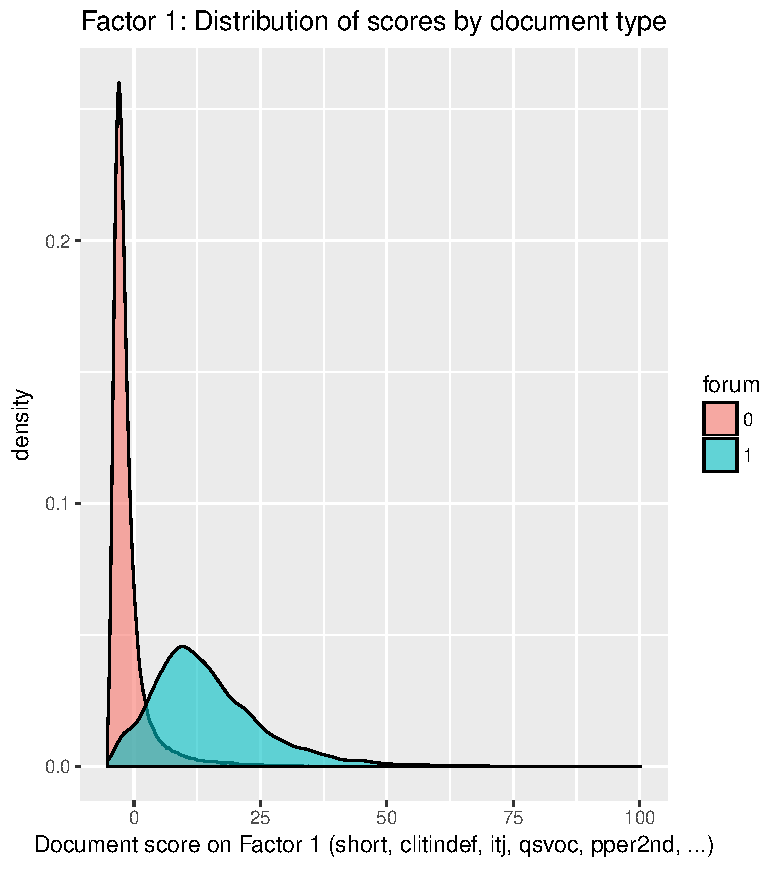
\includegraphics[scale=.95]{../R/forum-factor1.pdf}
   \label{forum-factor1}
  \caption{Distribution of factor scores (Factor~1). On average, forum documents show higher scores (14.6) than non-forum documents (-1.3). Prominent features on Factor~1 include short/contracted word forms, cliticised variants of the indefinite article, interjections, imperatives, 1st and 2nd person pronouns, emoticons, and words typical of informal written language.}  
\end{figure}

By generating factor scores for each of the 7 factors for each document, we have enriched our corpus with 7 additional meta data variables at the document level.
In the next section, we will use these variables as document-level predictors in a study on a specific syntactic alternation phenomenon, and compare the results to alternative models that use non-aggregated COReX counts as predictors.






\section{Case studies}
\label{sec:case-studies}
In this section, we explore the consequences of aggregating individual linguistic predictors into more abstract factors, for the purpose of modeling linguistic alternation phenomena.
In a \marginpar{series?}series of case studies, we model particular morpho-syntactic alternation phenomena with generalized linear models (GLMs), using different sorts of document-level information as predictors. For each case, we specify two alternative models, estimate the model coefficients, and compare these models wrt.\ to model fit and prediction accuracy:

\begin{enumerate}
  \item a model which uses as predictors the 7 factor scores from the factor analysis described in the previous section
  \item a model which uses as predictors the set of individual COReX features
\end{enumerate}

We are aware that these linguistic phenomena could probably be better explained / modeled if other kinds of predictors were taken into account as well (e.\,g., lexical information, syntactic properties at various levels).
However, since we are interested in what different sorts of document-level information can contribute to modeling the alternation phenomena, we deliberately ignore other predictors as part of our study design.



\subsection{Dative vs genitive case governed by prepositions}

A number of prepositions in German show variation wrt.\ case marking of their NP complement. A well-known example is the accusative/dative alternation after certain prepositions, which systematically encodes a semantic distinction (directional/non-directional; REF). Contrasting with this kind of semantically relevant alternation, some prepositions exhibit variation in case assignment which is not semantically motivated, but rather considered stylistic. The present case study focuses on the alternation between genitive and dative case, as illustrated in (\ref{prep-example1})--(\ref{prep-example4}).

\begin{exe}
  \ex \label{prep-example1}
    \begin{xlist}
      \ex trotz [starkem Verkehr]$_{dat}$\\
          `despite heavy traffic'
      \ex trotz [ihres Namens]$_{gen}$\\ 
          `despite her name'
    \end{xlist}
  \ex
  \begin{xlist}
    \ex wegen [dem Geschmack]$_{dat}$\\
        `because of the taste'
    \ex wegen [des besseren Aussehens]$_{gen}$\\ 
        `because of the better appearance' 
  \end{xlist}
  \ex
    \begin{xlist}
      \ex entgegen [dem urspr\"unglichen Gesetzentwurf]$_{dat}$\\
          `contrary to the original draft bill' 
      \ex entgegen [des Gesamttrends]$_{gen}$\\ 
          `contrary to the overall trend'
  \end{xlist}
  \ex \label{prep-example4}
    \begin{xlist}
        \ex gegen\"uber [einem Dritten]$_{dat}$\\
            `vis-à-vis a third party'
        \ex gegen\"uber [des Hotels]$_{gen}$\\ 
            `opposite the hotel' 
    \end{xlist}  
\end{exe}


 Typically, one of the variants is regarded as normative / canonical in Standard German, while the competing form has in many cases a non-standard flavour (see e.\,g., \citealp{Dimeola2009} and references therein).\footnote{For some prepositions, the normative case depends on morpho-syntactic properties of the complement NP. For instance, \textit{trotz} canonically assigns genitive, but dative is the only acceptable option with bare plural nouns which would otherwise lack a genitive inflectional ending. In what follows, we will only consider syntactic contexts where speakers/writers actually have a choice genitive and dative.} We therefore expect that the choice of case after these prepositions will depend, at least in part, on text type / genre, thus providing an ideal area for exploring the effects of feature aggregation. For the present case study, we selected a number of prepositions likely to exhibit some variation in dative/genitive case:
 
 \begin{quote} 
   abzüglich, angesichts, anlässlich, au{\ss}er, betreffs, bezüglich, dank, einschlie{\ss}lich, entgegen, gegenüber, gemä{\ss}, hinsichtlich, mangels, mitsamt, mittels, nebst, samt, seitens, trotz, vorbehaltlich, während, wegen, zuzüglich
 \end{quote}


We used the German web corpus DECOW16B \citep{SchaeferBildhauer2012} as well as the subset of the German reference corpus DeReKo \citep{Kupietz-ea2010} documented in\cite{BubenhoferKonopkaSchneider2014}. For each of these prepositions, all occurrences were extracted where the preposition is followed by either a determiner or an adjective that unambiguously mark dative or genitive case (cf. examples 1 and 8 above). Concordance lines from documents containing less than 100 tokens were discarded, so as to ensure that document-level feature counts are reasonably reliable. Moreover, we only kept a single instance per document, discarding all remaining instances. From this preliminary sample, we randomly selected 40,000 instances per corpus. Figure~\ref{genprops} shows the proportion of genitive complements by preposition and corpus.

\begin{figure}
   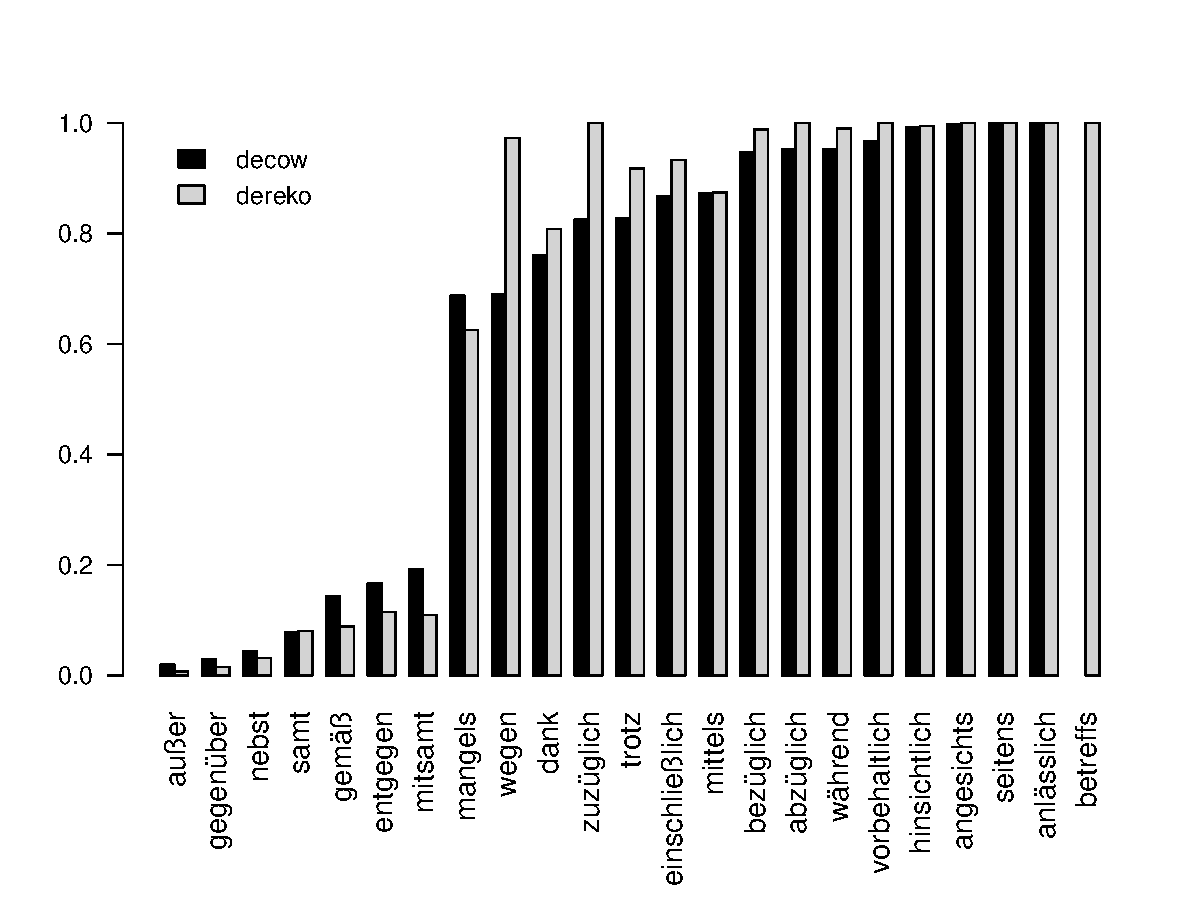
\includegraphics[scale=.7]{../R/prep-genitive-proportions}
   \label{genprops}
  \caption{Proportion of genitive complements (as opposed to dative) by preposition and corpus, in a sample of 80,000 prepositional phrases from DeReKo and DECOW16B}  
\end{figure}


A fair number (but by no means all) of the selected prepositions show some degree of variation in case assignment. For our final dataset, we selected only those prepositions where the proportion of either genitive or dative ocurrences was between 0.1 and 0.9 in at least one of the corpora. In other words, the amount of variation must be such that at least 10\% of all occurrences of that preposition show the minority, non-modal (and arguably, non-standard) case category. Thus, from among the original 23 prepositions, only 10 were included in the final dataset (\textit{entgegen}, \textit{gem\"a\ss}, \textit{mitsamt}, which typically select a dative complement, as well as \textit{dank}, \textit{einschlie{\ss}lich}, \textit{mangels}, \textit{mittels}, \textit{trotz}, \textit{wegen} and \textit{zuz\"uglich}, which typically select genitive). For this dataset, the overall occurence rate of non-standard case assignment is 15.4 \%.

We first specify two logistic regression models that predict the probability of observing the non-modal/non-standard case category, and which do not distinguish between individual prepositions. First, we use the set of COReX variables, represented as $c_1$ \ldots $c_{60}$ in equation~\ref{glm-allpreps-corex}.

\marginpar{Variable name}
\begin{equation}
\label{glm-allpreps-corex}
  P(nonstandard.case=1) = logit^{-1}(\alpha + \beta_1 c_1 + \beta_2 c_2 + \dots + \beta_{60} c_{60})
\end{equation}


Of the resulting coefficient estimates, 32 are different from 0 at p < 0.05. The Nagelkerke Pseudo-R$^2$ score for this model is 0.28.

For comparison, we use the document factor scores from the factor analysis as shown in equation~\ref{glm-allpreps-fa} (where the terms $f_1$ \ldots $f_7$ represent the factor scores of factors 1 through 7). In this model, all coefficient estimates are significant at the 0.05 level, however, the Nagelkerke R$^2$ score for this model drops to 0.24.

\marginpar{Matrizenoder Laufindex oder Fußnote und erklären}
\begin{equation}
\label{glm-allpreps-fa}
  P(nonstandard.case=1) = logit^{-1}(\alpha + \beta_1 f_1 + \beta_2 f_2 + \dots + \beta_{7} f_{7})
\end{equation}


Next, we consider separate models for each preposition, using all 60 COReX features as predictors. Figure~\ref{coeffs-corex-individial} illustrates the distribution of estimates for each preposition, for each coefficient with an associated p-value < .05 and absolute value < 5. As is obvious from the plot, coefficient estimates vary greatly, depending on the preposition. 

\begin{figure}
  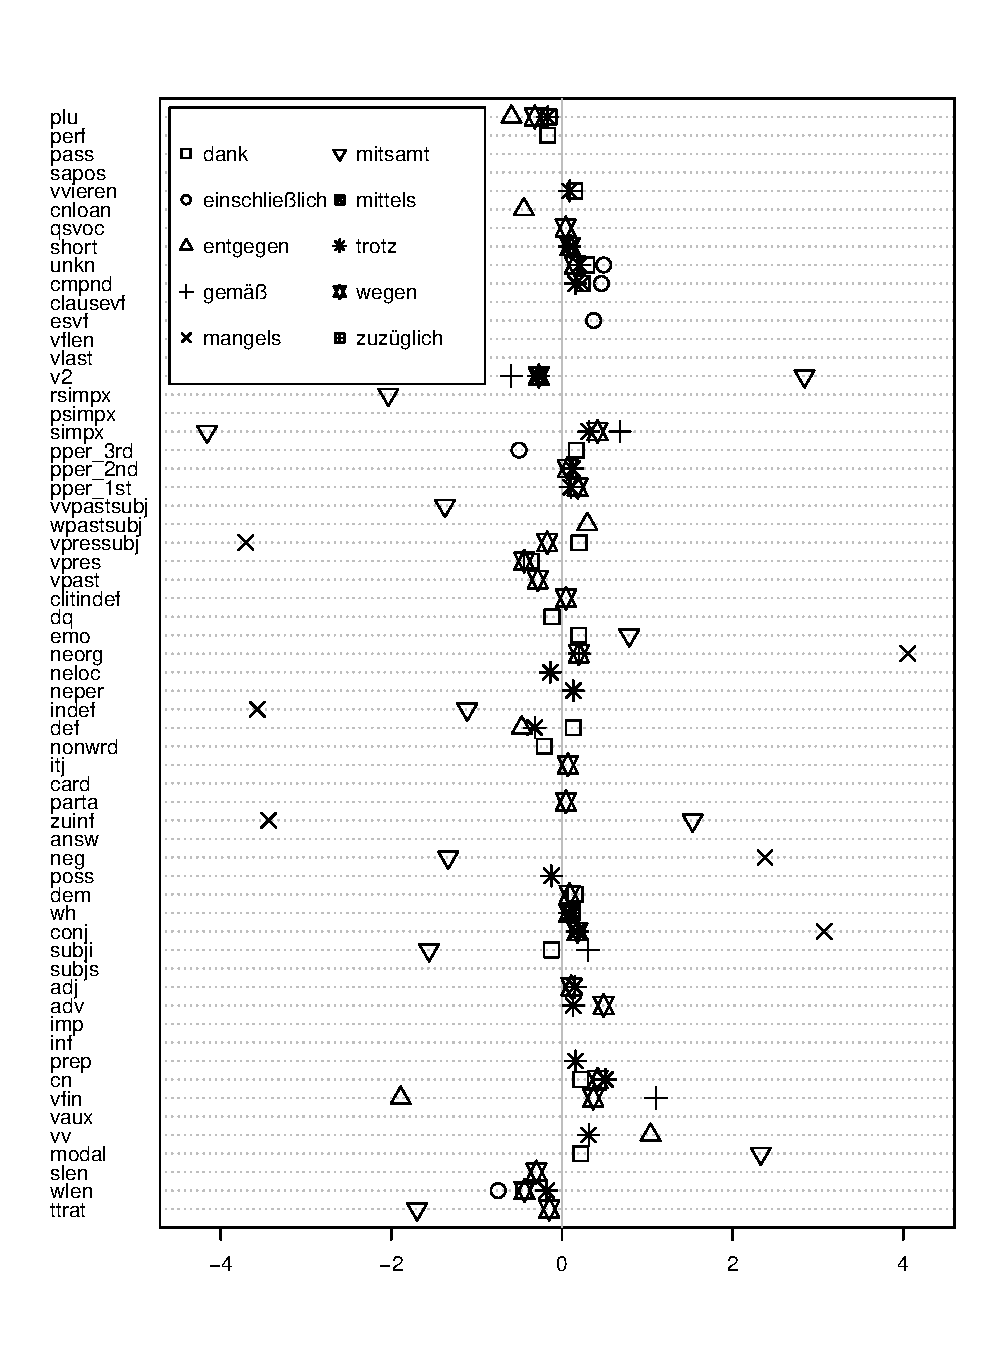
\includegraphics[scale=.9]{../R/prep-individual-coeffs-bw}
  \label{coeffs-corex-individial}
  \caption{COReX features: coefficient estimates with associated p-value $< 0.05$; a separate model was specified for each preposition.}
\end{figure}



\printbibliography
\end{document}
